\section{Biblioteca RailML}
	\label{sec:Biblioteca}
	
    El primer paso en el desarrollo del RNA es contar con una librería que permita generar un objeto equivalente uno a uno con el estándar railML y luego exportar un nuevo archivo railML. Como ya se mencionó en la Sección \ref{sec:railML}, el estándar railML define cinco clases de objetos principales: Common, Infraestructure, Interlocking, RollingStock y Timetable. 

    La clase Common incluye 109 subclases, todas ellas utilizadas para definir características generales e invariantes para la red. Por ejemplo, podemos encontrar la clase Concessionaire que define quien tiene la concesión de la red, la clase tBrakeType que define el tipo de frenos aceptados en esa red, la clase tVoltage que define la tensión de la red o la clase PublicHolidayPeriodRule que define el período de vacaciones de los operarios de la red, entre otros factores. Esta clase es obligatoria para todos los archivos en formato railML, por lo tanto es necesaria para el funcionamiento del RNA, aunque no se extraigan datos importantes de la misma.

    La clase Infraestructure incluye  231 subclases, todas ellas enfocadas en definir las características estáticas de cada elemento ferroviario, como su posición, dimensiones y demás parámetros invariantes en el tiempo.  Entre ellas podemos encontrar la clase Borders (ver Sección XX), BufferStops (ver Sección XX), LevelCrossingsIS (ver Sección XX), Platforms (ver Sección XX), SignalsIS (ver Sección XX), SwitchesIS (ver Sección XX) y Tracks (ver Sección XX), entre otras. Adicionalmente incluye dos clases fundamentales para el análisis de redes de grafos: netElement y netRelation, ambas discutidas en la Sección XX. En el caso de hacer análisis a nivel meso y macroscópico se tienen, además, las clases Line, OperationalPoint y Network, no cubiertas en este análisis.

    La clase Interlocking incluye 156 subclases, todas ellas enfocadas en definir las características dinámicas de los elementos ferroviarios que las posean. Entre ellas podemos encontrar LevelCrossingsIL (ver Sección XX), SignalsIL (ver Sección XX), SwitchesIL (ver Sección XX), entre otras. Adicionalmente, se encuentras las subclases relacionadas a la tabla de enclavamientos y las rutas, como Routes, CombinedRoutes, ConflictingRoutes, RoutesRelations y muchas otras referidas explícitamente a rutas (ver Sección XX). 
    
    El RNA solamente necesita de las clases Common, Infraestructure e Interlocking para funcionar, por lo que no fue necesario implementar las clases RollingStock ni Timetable. En total se han implementado 524 clases, considerando 28 clases nativas de RailTopoModel necesarias para que railML pueda interpretar los tipos de datos definidos. Todas las clases y subclases mencionadas son opcionales en el estándar, salvo que se indique lo contrario, es decir, no son obligatorias para que el archivo railML se considere válido.

    En las siguientes secciones se detallaran las subclases mas importantes implementadas, tal que se pueda comprender que atributos son procesados para poder generar el señalamiento. Se comenzará con las clases relativas a la topología de la red, eje central análisis del RNA y se proseguirá con las clases asociadas a elementos ferroviarios materiales. Simultáneamente, se profundizará en los conceptos mas destacados de cada elemento ferroviario correspondiente a esa clase, destacando cual es el señalamiento asociado al mismo para protegerlo en base a los principios ferroviarios expuestos.

    % COMMON
    \subsection{Clase \textit{Metadata}}
    \label{sec:metadata}

    Aunque no es una clase de railML, la clase \textit{Metadata} es fundamental para que el archivo en formato railML sea válido. Se presenta el Código \ref{lst:metadata} para ilustrar los elementos presentes en la clase metadata.
    
    \begin{lstlisting}[language = XML, caption = Clase \textit{Metadata}, label = {lst:metadata}]
<metadata>
    <dc:title>Example_9.railml</dc:title>
    <dc:date>2023-10-04T10:51:21Z</dc:date>
    <dc:creator>Trenes_Argentinos</dc:creator>
    <dc:source>RaIL-AiD</dc:source>
    <dc:identifier>1</dc:identifier>
    <dc:subject>railML.org</dc:subject>
    <dc:format>0.9.5</dc:format>
    <dc:description>Ejemplo_real</dc:description>
    <dc:publisher>RaIL-AiD framework</dc:publisher>
</metadata>
    \end{lstlisting}

    Ninguno de estos campos es esencial para el análisis de la red ferroviaria, por lo que son copiados sin cambios al nuevo archivo generado. No obstante, la ausencia de alguno de estos campos o que el campo sea nulo provoca que tanto el RNA como cualquier herramienta compatible con railML considere al archivo como incompleto o corrupto.
    \subsection{Clase common}
    \label{sec:common}

    La clase Common define todos los parámetros que son invariantes a toda la red. Esta clase puede ser definida solo una vez o no definirse. Sus clases son:

    \begin{itemize}
        \item ElectrificationSystems: define la tensión y frecuencia de la red eléctrica.
        \item OrganizationalUnits: define quien administra la infraestructura, quien fabrica y opera el material rodante, quien es el cliente final, quien es el contratista y quien posee la concesión del servicio. 
        \item SpeedProfiles: define el perfil de aceleración, velocidades y frenado.
        \item Positioning: define los sistemas de posicionamiento geométrico, linear y referido a la pantalla del editor.
    \end{itemize}

    Cada uno de sus campos internos es único, pero también son opcionales. A modo de ejemplo se muestra el Código \ref{lst:common}, donde se ilustra como no todas las clases han sido definidas.
    
    \begin{lstlisting}[language = XML, caption = Clase Common , label = {lst:common}]
<common id="co_01">
    <organizationalUnits>
        <infrastructureManager id="im_01"/>
    </organizationalUnits>
    <positioning>
        <geometricPositioningSystems>
            <geometricPositioningSystem id="gps01">
                <isValid from="2023-07-26" to="2024-07-26"/>
                <name name="Example_9.railml" language="en"/>
            </geometricPositioningSystem>
        </geometricPositioningSystems>
        <linearPositioningSystems>
            <linearPositioningSystem linearReferencingMethod="absolute" 
            startMeasure="0" endMeasure="0" units="Km" id="loc-1">
                <isValid from="2023-07-26" to="2024-07-26"/>
                <name name="Loc-1" language="en"/>
            </linearPositioningSystem>
        </linearPositioningSystems>
    </positioning>
</common>
    \end{lstlisting}

    Solamente los clases OrganizationalUnits y Positioning fueron definidas, pero tanto el RNA como el estándar railML en el que el RNA se basa consideran válido a este fragmento de código. Los vectores son definidos en plural, como en el caso de geometricPositioningSystems cuyo primer, y único elemento en este caso, es geometricPositioningSystem con id="gps01". Es habitual ver estos vectores a lo largo de todo el archivo y será esencial poder determinar su dimensión para procesar correctamente los datos y contar la cantidad de elementos.

    
    % GRAFOS
    \subsection{Infraestructura y Redes de grafos}
    \label{sec:grafos}

    La clase Infraestructure define todos los elementos ferroviarios con características físicas, materiales y estáticas. Las subclases que contiene son:

    \begin{itemize}
        \item Topology: define la topología de la red mediante las subclases netElements y netRelationships. Incluye también la subclase Network para cumplir con el estándar de RailTopoModel.
        \item Geometry: define el sistema geométrico utilizado entre las subclases HorizontalCurve (en base al largo y el ángulo formado), GradientCurves (en base al largo y al gradiente ded la curva) y GeometryPoints (en base a una combinación de las dos subclases anteriores).
        \item FunctionalInfrastructure: define todos los elementos ferroviarios que el RNA analizará.
        \item PhysicalFacilities: actualmente el estándar lo define vacío, sin ninguna subclase interna salvo la subclase Any que puede ser utilizada como comodín.
        \item InfrastructureVisualizations: define las coordenadas y estructura del elemento ferroviario en base a sus subclases tRef (para indicar a que elemento afecta), SpotProjection (coordenada del elemento), LinearProjection (en caso de ser un elemento lineal) y AreaProjection (en caso de ser un elemento bidimensional).
        \item InfrastructureStates: define la validez de los datos referidos a cada elemento ferroviario.
    \end{itemize}

    Para realizar el análisis de la red, el RNA debe centrarse en tres de estas subclases: Topology (para conocer COMO es la red), FunctionalInfrastructure (para conocer QUE elementos tiene la red) y InfrastructureVisualizations (para conocer DONDE está cada elemento ferroviario).

    Empezando por la clase Topology, existen dos subclases esenciales para este análisis: la subclase netElements y la subclase netRelationships. Ambas son subclases vectores, constituidas por subclases mas pequeñas: netElement y netRelationship. Un ejemplo de la clase netElement se puede ver en el Código \ref{lst:netElement}.
    
    \begin{lstlisting}[language = XML, caption = Clase netElement , label = {lst:netElement}]
<netElement id="ne3">
    <associatedPositioningSystem id="ne3_aps01">
        <intrinsicCoordinate intrinsicCoord="0" id="ne3_aps01_ic01">
            <geometricCoordinate x="9384.050" y="0.000" positioningSystemRef="gps01"/>
        </intrinsicCoordinate>
        <intrinsicCoordinate intrinsicCoord="1" id="ne3_aps01_ic02">
            <geometricCoordinate x="7584.770" y="0.000" positioningSystemRef="gps01"/>
        </intrinsicCoordinate>
    </associatedPositioningSystem>
    <relation ref="nr_ne3ne46_swi77"/>
    <relation ref="nr_ne3ne53_swi77"/>
</netElement>
    \end{lstlisting}
    
    Los elementos mas importantes a destacar en el Código \ref{lst:netElement} son el id, el geometricCoordinate y el relation. De estos parametros podemos saber que el netElement es referido como "ne3", comienza en la coordenada (9384.050 ; 0.000) y termina en la coordenada (7584.770 ; 0.000). Además, ne3 se encuentra relacionado a los netElement ne46 y ne53 mediante un elemento referido como swi77, que mas adelante veremos que se trata de una máquina de cambios.

    Los netElement son los nodos de la red de grafos, pero estos no son puntuales, sino que son bidimensionales. De las coordenadas de ne3 podemos deducir que ne3 se encuentra definido de derecha a izquierda. Conocer la orientación del netElement será importante a la hora de definir la circulación, información necesaria para generar las rutas.

    La subclase netRelation son las aristas de la red de grafos que relacionan dos netElements entre si. En el Código \ref{lst:netRelation} se muestra un ejemplo de los netRelation que vinculan a los netElement ne3, ne46 y ne53.    
    
    \begin{lstlisting}[language = XML, caption = Clase netRelation , label = {lst:netRelation}]
<netRelation navigability="Both" positionOnA="1" positionOnB="1" id="nr_ne3ne46_swi77">
    <elementA ref="ne3"/>
    <elementB ref="ne46"/>
</netRelation>
<netRelation navigability="Both" positionOnA="1" positionOnB="1" id="nr_ne3ne53_swi77">
    <elementA ref="ne3"/>
    <elementB ref="ne53"/>
</netRelation>
<netRelation navigability="None" positionOnA="1" positionOnB="1" id="nr_ne46ne53_swi77">
    <elementA ref="ne46"/>
    <elementB ref="ne53"/>
</netRelation>
    \end{lstlisting}
    
    La primer netRelation es entre el netElement ne3 y el ne46, la segunda netRelation es entre el netElement ne3 y el ne53. Esto es consistente con los parámetros de relation que tenía el netElement ne3 en el Código \ref{lst:netElement}. Sin embargo, en el tercer netRelation vemos que existe una relación entre los netElement ne46 y ne53 pero, en este caso, el parámetro navigability es "None", a diferencia de los primeros dos que era "both". La navegabilidad es el parámetro que hace que una red de grafos tenga sentido como red ferroviaria: que exista una conexión no implica que sea físicamente utilizable por un tren, tal como se explico en la Sección \ref{sec:RTM}.
    
    % Explicar analisis de red de grafos


        \begin{algorithm}\captionsetup{labelfont={sc,bf}, labelsep=newline}
            \caption{Graph network analysis algorithm}
            \label{alg:graph_network}
            \begin{algorithmic}
                \STATE \{nodes\} $\gets$ get\_nodes(netElements)
                \STATE  order\_nodes(\{nodes\})
                \STATE \{netPaths\} $\gets$ get\_relations(\{nodes\},netRelations)
                \STATE \{neighbours\} $\gets$ get\_neighbours(\{netPaths\})
                \STATE \{switches\} $\gets$ get\_switches(\{nodes\},\{neighbours\})
                \STATE \{limits\} $\gets$ get\_limits(\{nodes\})
                \STATE analyze\_connectedness(\{netPaths\})
            \end{algorithmic}
        \end{algorithm}


\begin{algorithm}\captionsetup{labelfont={sc,bf}, labelsep=newline}
            \label{alg:connectedness}
            \caption{Connectivity algorithm}
            \begin{algorithmic}
                \STATE \{zones\} $\gets \{ \}$
                \STATE ADD first node in \{zones\}
                \FOR {node in \{nodes\}}
                    \FOR {zone in \{zones\}}
                        \IF {node not in zones[zone]}
                            \IF {neighbours(node) in zones[zone]}
                                \STATE zones[zone] ADD node
                            \ELSE
                                \STATE Define new\_zone
                                \STATE zones[new\_zone] ADD node
                            \ENDIF
                        \ENDIF
                    \ENDFOR
                \ENDFOR 
            \RETURN \{zones\}
            \end{algorithmic}
        \end{algorithm}

    \begin{algorithm}\captionsetup{labelfont={sc,bf}, labelsep=newline}
            \caption{Switches detector algorithm}
            \label{alg:switches}
            \begin{algorithmic}
                \STATE \{switches\} $\gets$ \{\}
                \IF {infrastructure.SwitchesIS != None} 
                    \FOR{i in infrastructure.SwitchesIS[0].SwitchIS}
                        \IF{i.Id not in switchesIS.keys()}
                            \STATE sw\_id $\gets$ i.Name[0].Name
                            \STATE j $\gets$ i.SpotLocation[0]
                            \STATE left\_id $\gets$ i.LeftBranch[0].NetRelationRef
                            \STATE right\_id $\gets$ i.RightBranch[0].NetRelationRef
                            \STATE switches[sw\_id] $\gets$ \{"Node":j.NetElementRef\}
                            \STATE switches[sw\_id] $\gets$ \{"Continue":i.ContinueCourse\}
                            \STATE switches[sw\_id] $\gets$ \{"Branch":i.BranchCourse\}
                            \STATE switches[sw\_id] $\gets$ \{"Dir":j.ApplicationDirection\}
                            \STATE switches[sw\_id] $\gets$ \{"LeftBranch":j.left\_id\}
                            \STATE switches[sw\_id] $\gets$ \{"RightBranch":j.right\_id\}
                        \ENDIF
                    \ENDFOR
                \ENDIF
                \STATE visual\_data $\gets$ visualization.Visualization
                \IF {visual\_data != None}
                    \FOR {i in  visual\_data[0].SpotElementProjection}
                        \STATE sw\_id $\gets$ i.Name[0].Name
                        \IF {"Sw" in sw\_id}
                            \STATE pos\_x $\gets$ int(i.Coordinate[0].X)
                            \STATE pos\_y $\gets$ int(i.Coordinate[0].Y)
                            \STATE switches[sw\_id] $\gets$ \{"Position":[pos\_x,-pos\_y]\}
                        \ENDIF 
                    \ENDFOR
                \ENDIF
            \RETURN switchesIS
            \end{algorithmic}
        \end{algorithm}

    %% Identificar nodos y aristas
    %% Identificar orientaciones
    %% Detectar conexidad
    %% Detectar si es una red ferroviaria o no


    \begin{algorithm}[hbt!]
        \caption{Level crossing algorithm}\label{alg:LC}
        \DontPrintSemicolon
        %\SetAlgoLined
        \SetNoFillComment
        \LinesNotNumbered 
        \For { netElement WITH LevelCrossing }
        {
            \tcc{Before reaching level crossing}
            [Signals] $\gets$ ADD circulation signal $>>>$\;
            \tcc{After leaving level crossing}
            [Signals] $\gets$ ADD circulation signal $<<<$\;
        }
        \KwResult{[Signals]} 
    \end{algorithm}



    
    
    En las siguientes subsecciones se analizaran en conjunto los elementos ferroviario descriptos en las subclases FunctionalInfrastructure y InfrastructureVisualizations.
    
     % ELEMENTOS
    \subsection{Vías}
	\label{sec:tracks}
	
    Las vías férreas son el elemento ferroviario mas esencial, son la columna vertebral de la infraestructura ferroviaria. Estas constituyen el sitio por el cual se desplazan los trenes, definiendo no solo la dirección del desplazamiento, sino también restringiendo el dominio del tren. Esto lo diferencia de otros medios de transporte como el automóvil que, aún teniendo una carretera, puede moverse por fuera de esta.

    Las vías se encuentran separadas por una distancia fija que se mide desde sus caras internas, denominada trocha (Figura \ref{fig:vias_1}). Solamente las formaciones compatibles con ese parámetro de trocha pueden circular por el tendido ferroviario. El valor de la trocha puede variar entre las denominadas trocha angosta (600 a 1372 mm, estándar imperial británico) y trocha ancha (1520 a 2140 mm, estándar ruso, indio, ibérico, irlandés). Se estableció el valor intermedio de 1435 mm como valor de trocha internacional, usado ampliamente en Europa, Norteamérica y Oceanía.

    \begin{figure}[H]
        \centering
        \includegraphics[width=1\textwidth]{Figuras/trocha.png}
        \centering\caption{Vías ferroviarias y trocha.}
        \label{fig:vias_1}
    \end{figure}
    
    Existen limitaciones logísticas y físicas por las cuales el tendido ferroviario no puede ser un continuo rígido. En primer lugar, las vías deben ser de un tamaño acotado, tal que puedan transportarse a la locación donde serán instaladas en tramos rectos o curvos. En segundo lugar, la dilatación y contracción de las vías debido a los cambios de temperatura añaden una restricción respecto a la distancia mínima que deben tener entre las mismas. De lo contrario, la dilatación del material puede provocar daños irreparables a la infraestructura y estos, a su vez, ser motivo de descarrilamientos, como ya ha ocurrido en los comienzos de la industria ferroviaria \cite{ACCIDENTE}. 
    
    Cada vía puede ser clasificada en dos grupos: vías ascendentes o vías descendentes (ver Figura \ref{fig:vias_2}). Las ascendentes son aquellas por las cuales los trenes circulan únicamente en la dirección del kilometraje en sentido creciente. Las descendentes son aquellas por las cuales los trenes circulan únicamente en la dirección del kilometraje en sentido decreciente \cite{RITO}. 

    \begin{figure}[H]
        \centering
        \includegraphics[width=1\textwidth]{Figuras/ascDesc.png}
        \centering\caption{Vías ascendentes y descendentes.}
        \label{fig:vias_2}
    \end{figure}

    El kilómetro cero es la estación principal de la línea ferroviaria, como pueden ser las terminales de Plaza Constitución (para la línea Roca), Once de septiembre (para la línea Sarmiento) y Retiro (para las líneas Mitre y San Martín).  Existen vías de maniobra que pueden ser tanto ascendentes como descendentes. Estas vinculan, mediante un cambio de vías, una sección ascendente con otra descendente, en la cual los trenes deben circular a una velocidad reducida. 

    Las vías se agrupan en secciones que, por cuestiones de seguridad y logística, se establece que solo pueden ser utilizadas por un tren a la vez. Estas secciones pueden ser de varios kilómetros en zonas rurales o unos pocos cientos de metros en zonas urbanas, donde la red necesita una mayor granularidad debido a la densidad del tráfico ferroviario en las grandes urbes.

    En railML las vías son elementos ferroviarios físicos, representados por la clase track, ilustrada en el Código \ref{lst:track}. Esta clase se encuentra definida dentro del vector de clases tracks, dentro de la clase functionalInfrastructure, dentro de la clase infrastructure.

    \begin{lstlisting}[language = XML, caption = Clase track , label = {lst:track}]
    <track type="mainTrack" infrastructureManagerRef="im_01" mainDirection="both" id="trk2">
        <trackBegin ref="bus5"/>
        <trackEnd ref="swi77"/>
        <length value="1799.28" type="physical"/>
        <designator register="_Example" entry="TRACK track2"/>
        <linearLocation applicationDirection="both" id="trk2_lloc01">
            <associatedNetElement netElementRef="ne3" keepsOrientation="true"/>
        </linearLocation>
        <name name="track2" language="en"/>
    </track>
    \end{lstlisting}
    
    Las vías en railML se definen entre dos elementos ferroviarios físicos. En este caso, la vía indicada como trk2 se encuentra definida entre el BufferStop bus5 (ver Sección \ref{sec:bufferstop}) y la máquina de cambios swi77 (ver Sección \ref{sec:switches}). Esta clase define, además, el largo de la vía y el netElement al cual están asociadas, en este caso, el netElement ne3. Es natural confundirse tracks y netElements, porque son términos casi equivalentes, pero un track representa un elemento físico y un netElement engloba de manera abstracta una porción del trazado de vías. Es decir, una vía puede dividirse en varios netElements, pero un netElement solo se asocia a una vía.
    \subsection{Fin de via}

\lipsum[1]
    \subsection{Sistemas de detección de formaciones ferroviarias}
    \label{sec:detectors}
    
    Es de vital importancia que el sistema pueda determinar la posición de un tren dentro del tendido ferroviario. De esta manera, poder habilitar la circulación en secciones donde no exista peligro de colisión con otros formaciones o, por el contrario, detener la marcha de las formaciones anteriores para evitar accidentes. Existen diversas maneras de detectar la posición de un tren, entre ellas el uso de circuitos de vía y contadores de ejes (Figura \ref{fig:deteccion_1}). 

    \begin{figure}[H]
        \centering
        \includegraphics[width=1\textwidth]{Figuras/detector}
        \centering\caption{Circuito de vía (01) y contador de ejes (AxC01).}
        \label{fig:deteccion_1}
    \end{figure}

    Los circuitos de vía (Figura \ref{fig:deteccion_2}) son dispositivos eléctricos que aplican una diferencia de potencial entre los rieles. Cuando una formación ingresa a la sección, sus ruedas metálicas cortocircuitan ambos rieles. El cortocircuito es detectado por el relé, que a su vez, reporta el estado al resto del sistema. 

    \begin{figure}[H]
        \centering
        \includegraphics[width=1\textwidth]{Figuras/circuitoVia}
        \centering\caption{Circuito de vía libre y ocupado.}
        \label{fig:deteccion_2}
    \end{figure}

    En caso de que la alimentación se interrumpa, el cableado sufra alguna falla, vandalismo, inundación, o que efectivamente una formación ocupe la sección, el circuito de vía reportará que la sección se encuentra ocupada. De esta manera, solo es posible recibir un reporte de sección desocupada cuando la sección efectivamente se encuentre desocupada. A este principio se le denomina fail-safe \cite{Paper_5,Paper_94,Paper_95,Paper_96}. Es decir, si por alguna razón algo falla, el sistema adopta la condición más restrictiva, mitigando la posibilidad de una situación peligrosa. 
    
    Existe una discontinuidad entre los rieles denominado juntura, que permite la expansión de los mismos al ser sometidos a altas temperaturas sin que los rieles se doblen y provoquen daños a la infraestructura. Los circuitos de vía, se relacionan directamente a las junturas entre las vías, modelados por la clase \textit{railJoint} en railML.  Esta discontinuidad eléctrica es lo que limita la acción del circuito de vía a la región entre dos junturas.

    En el código \ref{lst:trackCircuit} podemos ver un ejemplo de la clase \textit{tvdSection} dentro de la clase \textit{interlocking}, que incluye a la clase \textit{assetsForIL} y estos, a su vez, a la clase vector de \textit{tvdSections}. Esta clase posee un id (tvd7), la tecnología utilizada (en este caso \textit{trackCircuit}, circuito de vía) y los límites donde el circuito de vía es válido: los \textit{bufferStop} bus1 y bus2.

    \begin{lstlisting}[language = XML, caption = Clase \textit{TrackCircuit} , label = {lst:trackCircuit}]
    <tvdSection id="tvd7" partialRouteReleaseDelay="PT4S" residualRouteCancellationDelay="PT90S" technology="trackCircuit" isBerthingTrack="false">
        <designator register="Example" entry="01"/>
        <hasDemarcatingBufferstop ref="bus2"/>
        <hasDemarcatingBufferstop ref="bus1"/>
    </tvdSection>
    \end{lstlisting}

    Los sistemas contadores de ejes (Figura \ref{fig:deteccion_2}) consisten en sensores pasivos instalados en la cara interna de unos de los rieles y un sistema externo de procesamiento de datos. Estos sistemas no dependen de la aplicación de tensiones en la vía. Además, no solo permiten detectar la presencia de una formación, sino que también pueden usarse para medir la integridad de la formación, si se conoce a priori la cantidad de ejes de la misma. 

    \begin{figure}[H]
        \centering
        \includegraphics[width=1\textwidth]{Figuras/contador}
        \centering\caption{Contadores de ejes.}
        \label{fig:deteccion_2}
    \end{figure}

    Al igual que los circuitos de vía, los sistemas contadores de eje siguen el principio de fail-safe, adoptando la condición mas restrictiva en caso de falla. Ambos sistemas pueden utilizarse en simultáneo, de ser requerido. En el código \ref{lst:axleCounter} podemos ver un ejemplo de la clase \textit{trainDetectionElement}, dentro de la clase \textit{functionalInfrastructure}, dentro de la clase \textit{infrastructure}. En este ejemplo la bclase fue definida como tipo \textit{axleCounter} (contador de eje) y se le asigna el nombre AxC01 que vemos en la Figura \ref{fig:deteccion_1}, referido al \textit{netElement} ne1. También podemos ver que este contador de ejes se activa en ambos sentidos (applicationDirection = both) y su coordenada intrínseca dentro del \textit{netElement} ne1, dentro de los dos tercios de la sección.

    \begin{lstlisting}[language = XML, caption = Clase \textit{TrainDetectionElement} , label = {lst:axleCounter}]
    <trainDetectionElement id="ac6" type="axleCounter">
        <name name="AxC01" language="en"/>
        <spotLocation id="ac6_sloc01" netElementRef="ne1" applicationDirection="both" intrinsicCoord="0.6710"/>
        <designator register="Example" entry="TRAIN DETECTION ELEMENT AxC01"/>
    </trainDetectionElement>
    \end{lstlisting}
    %\subsubsection{Automatic Train Stop (ATS)}

\lipsum[1]

    \begin{figure}[!h]
        \centering
        \includegraphics[width=1\textwidth]{Figuras/ATS}
        \centering\caption{ATS.}
        \label{fig:ATS_1}
    \end{figure}

\lipsum[1]
    \subsection{Plataformas}

\lipsum[1]
    \subsection{Cruces de via}

\lipsum[1]
    \subsection{Cambios de vías}
    \label{sec:switches}
 	Un cambio de vías es un elemento ferroviario dinámico, que puede adoptar diferentes posiciones que modifican la topología de la red. Una formación por si sola no puede hacer mas que avanzar o retroceder, pero utilizando un cambio de vías es posible trazar nuevos caminos en el tendido ferroviario, modificando la posición de los cambios de vías.
 	
 	Los cambios de vías pueden ser simples, dobles o en tijeras. Las posiciones que pueden adoptar se visualizan en la Figura \ref{fig:cambios_0}. Un cambio de vías simple permite dos circulaciones posibles, una por vía principal y otra por vía secundaria. Un cambio de vías dobles permite cuatro circulaciones posibles, todas de igual prioridad. Un cambio de vías en tijeras permite dos circulaciones posibles, ambas principales.
 	
 	\begin{figure}[H]
 		\centering
 		\includegraphics[width=1\textwidth]{Figuras/circulacion.png}
 		\centering\caption{Circulaciones posibles en cambios de vías.}
 		\label{fig:cambios_0}
 	\end{figure}
 	
 	El sistema de enclavamientos modifica la posición de los cambios de vías por medio de una máquina de cambios. Una máquina de cambios (Figura \ref{fig:cambios_1}) es un mecanismo utilizado para permitir el paso de las formaciones de una vía a una ramificación del recorrido principal. Esto se realiza mediante el movimiento de la aguja del cambio (riel móvil) hacia su respectiva contraaguja (riel fijo) hasta obtener un adecuado acoplamiento que permita la circulación de la formación.

    \begin{figure}[H]
        \centering
        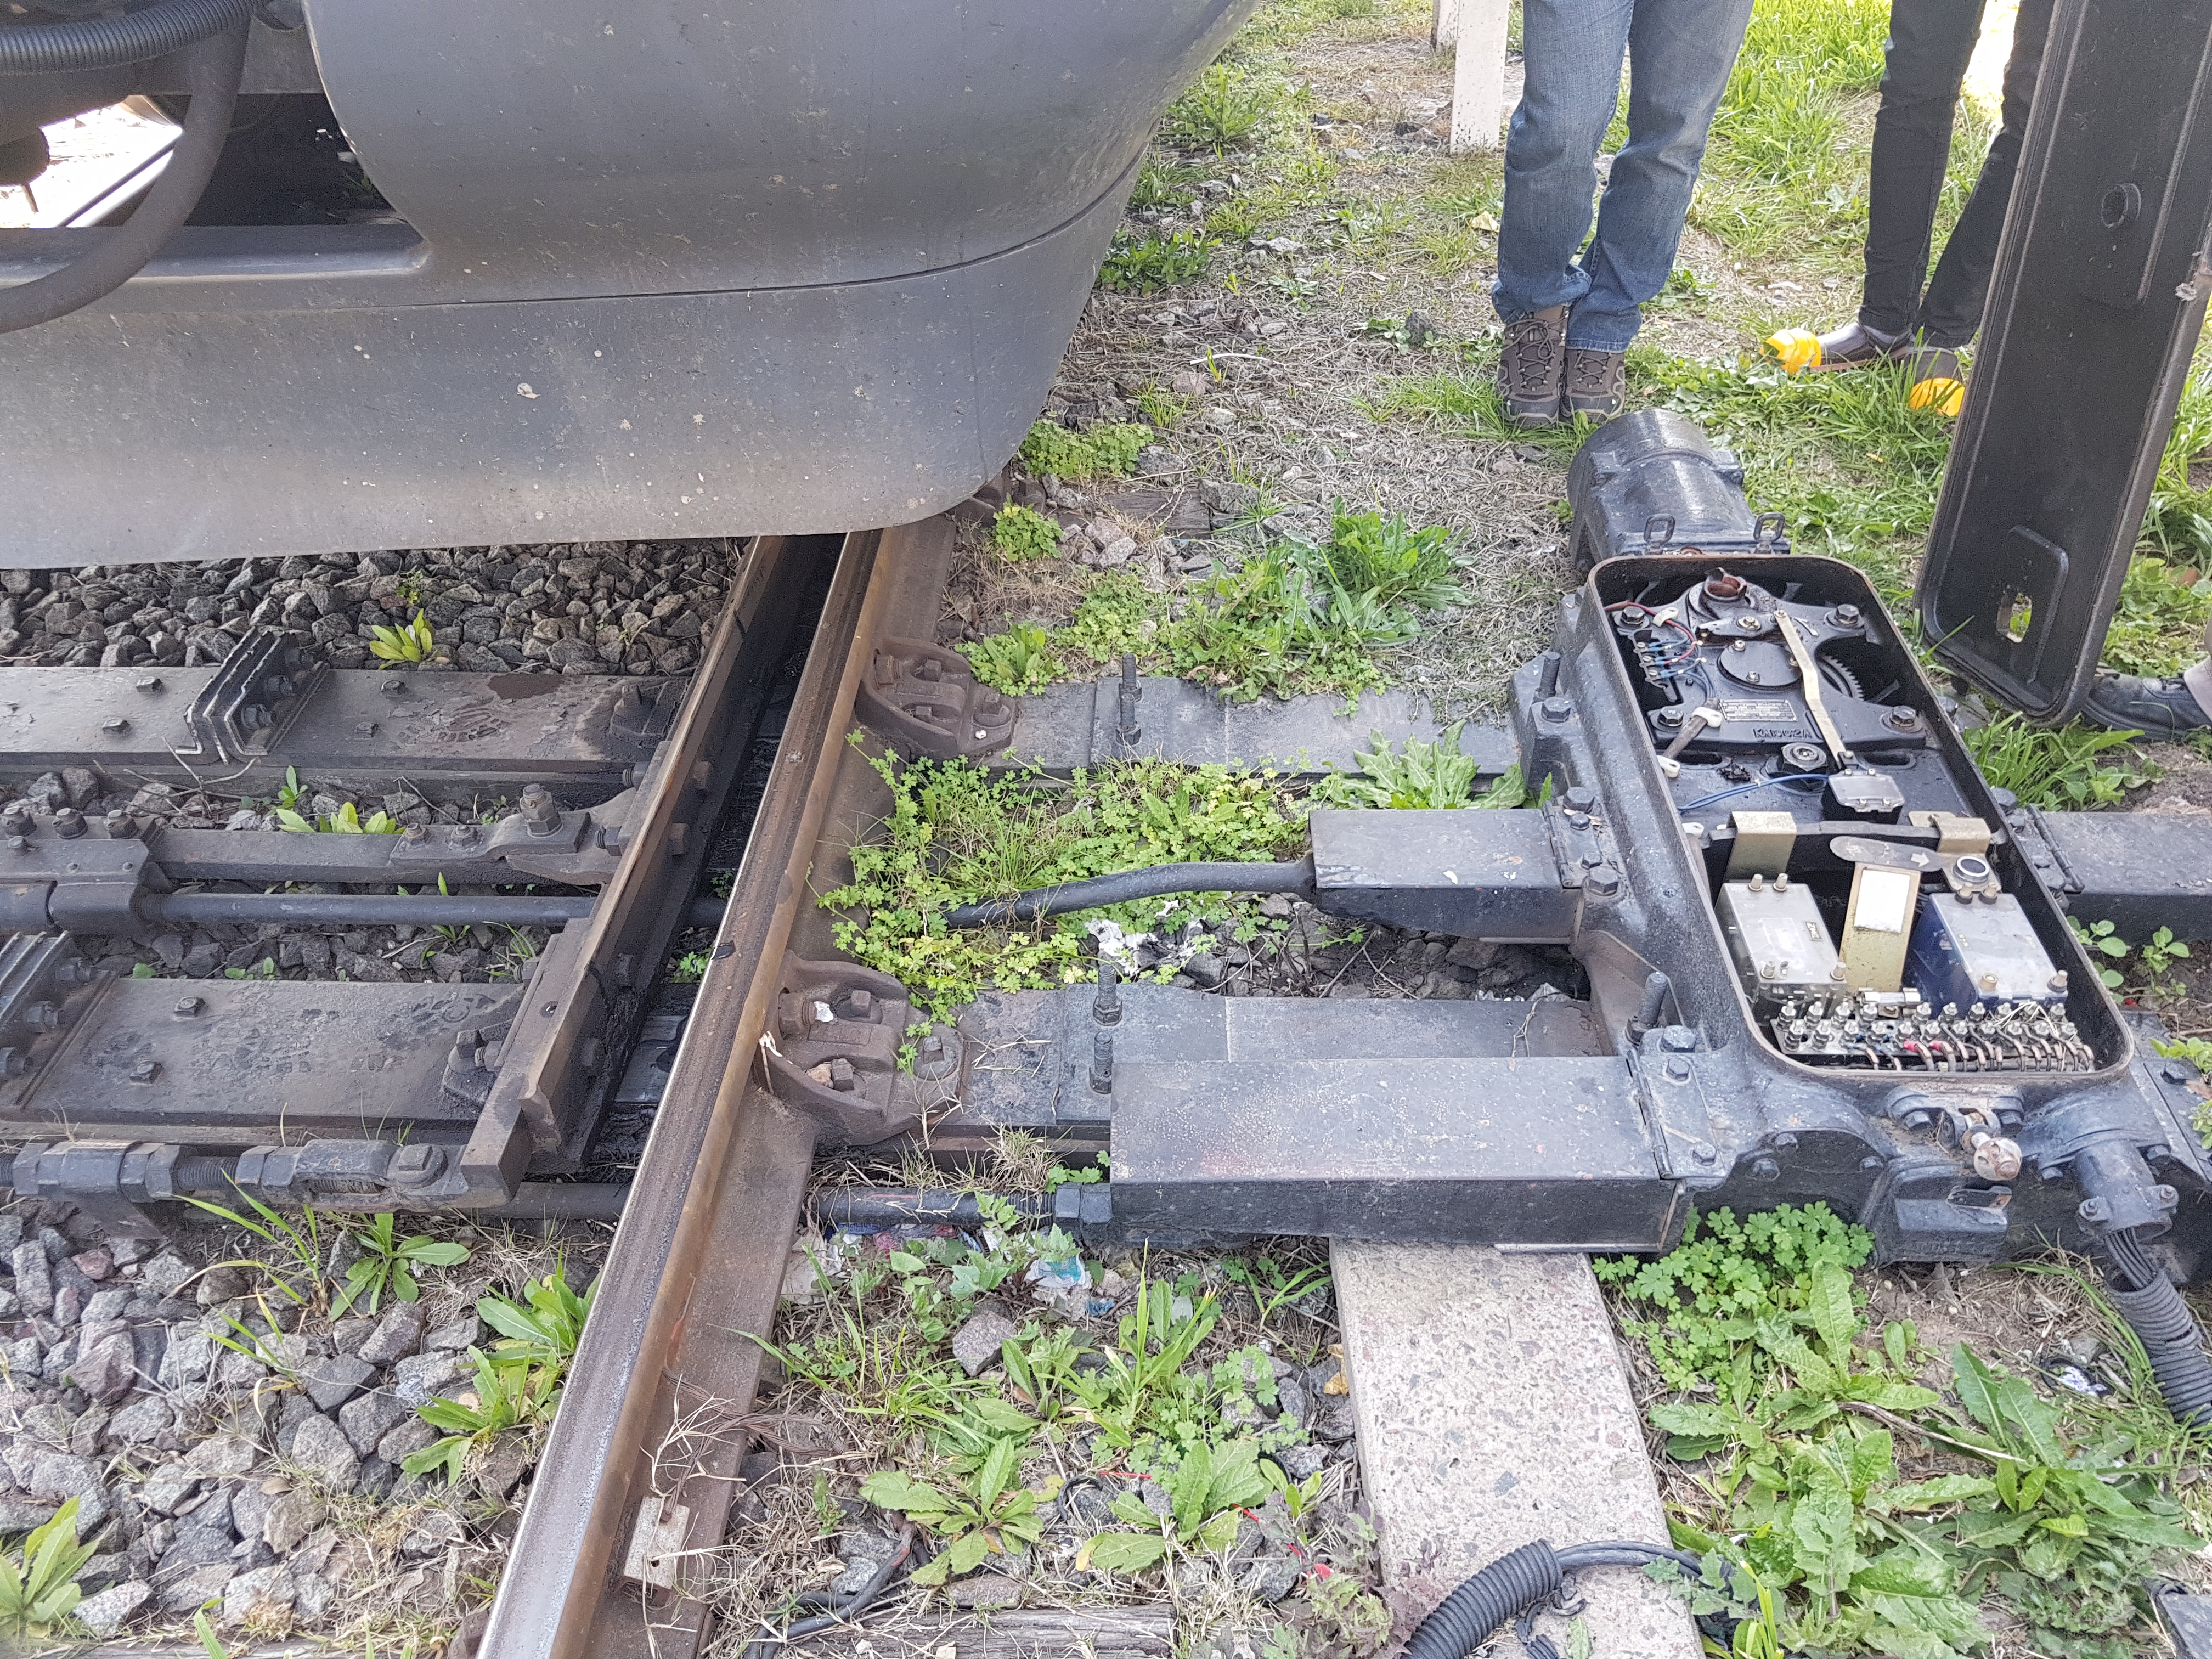
\includegraphics[width=0.75\textwidth]{Figuras/Cambios.jpg}
        \centering\caption{Máquina de cambios.}
        \label{fig:cambios_1}
    \end{figure}

    En la Figura \ref{fig:cambios_2} se muestra el cambio de vía de la estación Matheu de la Línea Mitre. Se observa que según sea la posición de la máquina de cambios, el tren puede continuar en la misma vía o hacer el cambio a la otra vía.

    \begin{figure}[H]
        \centering
        \includegraphics[width=0.75\textwidth]{Figuras/Cambios_2.jpg}
        \centering\caption{Cambio de vías de estación Matheu, Linea Mitre.}
        \label{fig:cambios_2}
    \end{figure}

    %En la Figura \ref{fig:cambios_3} se muestran las posiciones que puede adoptar el cambio. En la posición normal, los trenes pueden circular de forma directa, en paralelo, por la vía principal en sentidos opuestos. En la posición reversa, por el contrario, se permite el intercambio de trenes de una rama principal a otra en sentido opuesto o a una ramificación secundaria de la red.

   % \begin{figure}[H]
   %     \centering
   %     \includegraphics[width=1\textwidth]{Figuras/cambio_3.PNG}
   %     \centering\caption{Posiciones adoptadas por un cambio de vías simple.}
   %     \label{fig:cambios_3}
   % \end{figure}

    Al ser mecanismos que necesitan tiempo para cambiar de un estado al otro, no puede asumirse que el comando es obedecido al instante. Incluso podría darse el caso que jamás llegue a cumplirse la orden debido a desperfectos mecánicos o eléctricos. Es por eso que introducimos los conceptos de comando, indicación y correspondencia, tal como se ilustran en la Figura \ref{fig:cambios_4}.

    \begin{figure}[H]
        \centering
        \includegraphics[width=1\textwidth]{Figuras/cambios}
   \textit{}     \centering\caption{Comando, indicación y correspondencia en un cambio de vías.}
        \label{fig:cambios_4}
    \end{figure}
    
    El comando es la instrucción que el sistema de enclavamientos envía a la máquina de cambios. Esta instrucción puede ser modificar la posición de normal a reverso o de reverso a normal. La indicación es el estado que la máquina de cambios informa al sistema de enclavamientos. El sistema solo asume que el comando fue obedecido cuando tanto el comando como la indicación muestran una correspondencia. En caso contrario, el sistema de enclavamiento no puede asumir cual es el estado real del sistema, si el comando enviado o el estado reportado por la máquina de cambios. El mismo concepto puede ser aplicado en cualquier otro elemento mecánico, como por ejemplo las barreras ferroviarias.

    El RNA debe analizar diversos atributos distribuidos entre la clase \textit{switchIS} (Código \ref{lst:switchIS}), la clase \textit{spotElementProjection} (Código \ref{lst:switch}) y la clase \textit{switchIL} (Código \ref{lst:switchIL}). La clase \textit{switchIS} se encuentra dentro del vector de clases \textit{switchesIS}, dentro de la clase \textit{functionalInfrastructure}, que a su vez es parte de la clase infrastructure. La clase \textit{switchIS} define el id de la máquina de cambios, el tipo (ordinario), el \textit{netElement} al cual pertenece la entrada del cambio y hacia que lado se encuentra la vía de continuación y ramificación si transitamos desde el \textit{netElement} del cambio hacia el cambio mismo. En este caso, si transitamos por el \textit{netElement} ne16 el tren tendrá la vía de continuación en la mano derecha y la ramificación en la mano izquierda. Los cambios de vías simples ("ordinarySwitch") siempre tienen una rama izquierda y una rama derecha definida. Además, dentro de la definición de cada rama tenemos el atributo \textit{netRelationRef}, del cual se puede obtener, procesamiento mediante, los otros \textit{netElement} correspondientes a las ramas: ne15 y ne14.

    \begin{lstlisting}[language = XML, caption = Clase \textit{switchIS} , label = {lst:switchIS}]
    <switchIS id="swi84" continueCourse="right" branchCourse="left" type="ordinarySwitch">
        <name name="Sw01" language="en"/>
        <spotLocation id="swi84_sloc01" netElementRef="ne16" applicationDirection="reverse" intrinsicCoord="0.0000"/>
        <designator register="_Example" entry="SWITCH Sw01"/>
        <leftBranch netRelationRef="nr_ne15ne16_swi84" branchingSpeed="0" joiningSpeed="0" radius="-500"/>
        <rightBranch netRelationRef="nr_ne14ne16_swi84" branchingSpeed="0" joiningSpeed="0" radius="0"/>
    </switchIS>
    \end{lstlisting}

    La clase \textit{spotElementProjection} define la ubicación en el espacio del elemento ferroviario referido. En este caso, como se puede ver en el Código \ref{lst:switch}, la posición de la máquina de cambios es la coordenada (-561 ; -450).

    \begin{lstlisting}[language = XML, caption = Clase \textit{spotElementProjection} , label = {lst:switch}]
    <spotElementProjection refersToElement="swi84" id="vis01_sep16">
        <name name="Sw01" language="en"/>
        <coordinate x="-560.994" y="-450.000"/>
    </spotElementProjection>
    \end{lstlisting}

    La clase \textit{switchIL}, definida dentro del vector de clases \textit{switchesIL}, se encuentra dentro de la clase \textit{assetsForIL}, en la clase \textit{interlocking}. Contiene datos extra sobre el comportamiento dinámico del cambio de vías y define explícitamente los otros dos nodos, en contraposición a \textit{switchIS} del cual hay que obtenerlos procesando un string. El RNA puede obtener los \textit{netElement} de ambas clase y compararlos, anulando el análisis si los \textit{netElement} definidos en \textit{switchIS} y \textit{switchIL} no son coincidentes.
    
    \begin{lstlisting}[language = XML, caption = Clase \textit{SwitchIL} , label = {lst:switchIL}]
    <switchIL id="il_swi84" maxThrowTime="PT10S" typicalThrowTime="PT6S" isKeyLocked="false" returnsToPreferredPosition="false">
        <refersTo ref="swi84"/>
        <branchLeft ref="ne15"/>
        <branchRight ref="ne14"/>
    </switchIL>
    \end{lstlisting}
    
    El RNA utiliza el Algoritmo \ref{alg:switches} para detectar todos estos parámetros y crear un vector de máquinas de cambios (switches) indexado por el id de cada máquina de cambios (sw\_id). La existencia y ubicación de las máquinas de cambios ya se habían obtenido mediante el análisis de la red de grafos ferroviaria. El Algoritmo \ref{alg:switches} analiza la clase \textit{switchIS} y confirma la existencia de la máquina de cambios, para luego la clase \textit{spotElementProjection} y confirmar la ubicación de la misma. Los datos obtenidos en switches[sw\_id].LeftBranch y switches[sw\_id].RightBranch, permiten obtener los nodos de las ramificaciones que luego se conformarán analizando la clase \textit{switchIL} en algoritmos posteriores.

    \begin{algorithm}[H]\captionsetup{labelfont={sc,bf}, labelsep=newline}
            \caption{Algoritmo detector de cambios de vías.}
            \label{alg:switches}
            \begin{algorithmic}
                \STATE \{switches\} $\gets$ \{\}
                \IF {infrastructure.SwitchesIS != None} 
                    \FOR{i in infrastructure.SwitchesIS[0].SwitchIS}
                        \IF{i.Id not in switchesIS.keys()}
                            \STATE sw\_id $\gets$ i.Name[0].Name
                            \STATE j $\gets$ i.SpotLocation[0]
                            \STATE node $\gets$ j.NetElementRef
                            \STATE type $\gets$ i.Type
                            
                           	\IF{type == 'OrdinarySwitch'}
	                           	\STATE left\_id $\gets$ i.LeftBranch[0].NetRelationRef
	                           	\STATE right\_id $\gets$ i.RightBranch[0].NetRelationRef
	                           	\STATE switches[sw\_id] $\gets$ \{"Node":node\}
	                           	\STATE switches[sw\_id] $\gets$ \{"Continue":i.ContinueCourse\}
	                           	\STATE switches[sw\_id] $\gets$ \{"Branch":i.BranchCourse\}
	                           	\STATE switches[sw\_id] $\gets$ \{"Dir":j.ApplicationDirection\}
	                           	\STATE switches[sw\_id] $\gets$ \{"LeftBranch":j.left\_id\}
	                           	\STATE switches[sw\_id] $\gets$ \{"RightBranch":j.right\_id\}
                            \ENDIF
                            \IF{type == 'DoubleSwitchCrossing'}
	                            \STATE straightBranch\_A\_id $\gets$ i.StraightBranch[0].NetRelationRef
	                            \STATE straightBranch\_B\_id $\gets$ i.StraightBranch[1].NetRelationRef
	                            \STATE turningBranch\_A\_id $\gets$ i.TurningBranch[0].NetRelationRef
	                            \STATE turningBranch\_B\_id $\gets$ i.TurningBranch[1].NetRelationRef
	                            
	                            \FOR{X,Z combination(A,B)}
		                            \STATE switches[sw\_id+'XZ'] $\gets$ \{"Node":node\}
		                            \STATE switches[sw\_id+'XZ'] $\gets$ \{"Continue":i.ContinueCourse\}
		                            \STATE switches[sw\_id+'XZ'] $\gets$ \{"Branch":i.BranchCourse\}
		                            \STATE switches[sw\_id+'XZ'] $\gets$ \{"Dir":j.ApplicationDirection\}
		                            \STATE switches[sw\_id+'XZ'] $\gets$ \{"LeftBranch":j.straightBranch\_X\}
		                            \STATE switches[sw\_id+'XZ'] $\gets$ \{"RightBranch":j.turningBranch\_Z\}
	      						\ENDFOR
                            \ENDIF
                            
                        \ENDIF
                    \ENDFOR
                \ENDIF
                \STATE visual\_data $\gets$ visualization.Visualization
                \IF {visual\_data != None}
                    \FOR {i in  visual\_data[0].SpotElementProjection}
                        \STATE sw\_id $\gets$ i.Name[0].Name
                        \IF {'Sw' in sw\_id}
                            \STATE pos\_x $\gets$ int(i.Coordinate[0].X)
                            \STATE pos\_y $\gets$ int(i.Coordinate[0].Y)
                            \STATE switches[sw\_id] $\gets$ \{"Position":[pos\_x,-pos\_y]\}
                        \ENDIF 
                    \ENDFOR
                \ENDIF
            \OUTPUT \{switches\}
            \end{algorithmic}
        \end{algorithm}
    
    % SEMAFOROS
    \subsection{Semaforos}

\lipsum[1]